\section{Simulation results}
\label{simulation}
%\fabioBsays{if you already know how will be the video, you can describe it}

\subsection{Simulation Environment}

 %\begin{figure}[t]
 %     \centering
 %     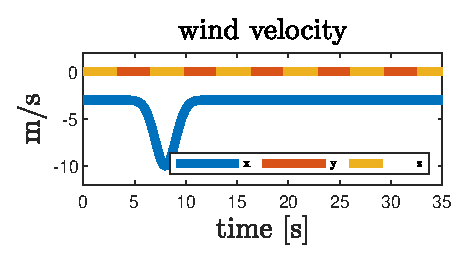
\includegraphics[width=60mm]{./imagines/wind_velocity_10.eps}
 %     \caption{Simulated air environment w.r.t. the inertial frame $\mathcal{I}$: ${}^{\mathcal{I}}\boldsymbol{v}_w$, $\boldsymbol{X}$ blue line, $\boldsymbol{Y}$ red line, $\boldsymbol{Z}$ yellow line} 
 %     \label{fig:wind}
%\end{figure}

The robot dynamics is simulated by numerically integrating the equations of motion with aerodynamic forces Eq.~\eqref{eq_motion_af} in a custom-made simulator implemented in MATLAB-Simulink. The controller is entirely designed in Simulink and runs at a frequency of $\SI{100}{Hz}$. A fast, inner torque control loop is designed to stabilize the joints velocities $\dot{s}$ towards the reference values generated with Eq. \eqref{eq:optimization_QP}.\looseness=-1

\subsection{Flight Envelope Design}

We designed a flight envelope composed as follows:

\begin{enumerate}
  \item \textit{Scenario 1}: the robot hovers in vertical position, while subject to a wind in the frontal direction that follows the profile depicted in Fig. \ref{fig:hovering_wind}. 
  \item \textit{Scenario 2}: the robot hovers and climbs to gain altitude, then moves forward at around $\SI{11}{m/s}$, in presence of a lateral wind with the profile of Fig. \ref{fig:high_speed_wind}.
\end{enumerate}
%
The wind profiles are composed of a constant wind of $\SI{3}{m/s}$, and wind gusts of different shapes with magnitude of $\SI{10}{m/s}$ and $\SI{15}{m/s}$ \cite{aero,wind,KAI2019108491}. 
%Fig. \ref{fig:scen} shows the robot flying during one of the scenarios described by the flight envelope.

%\begin{figure}[t]
%    \centering
%        \subfigure[]{\label{}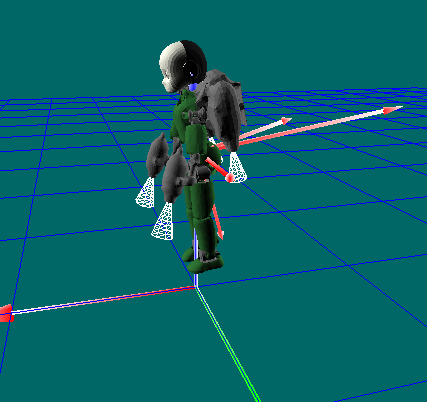
\includegraphics[width=30mm]{./imagines/arrow.png}}
%        \subfigure[]{\label{}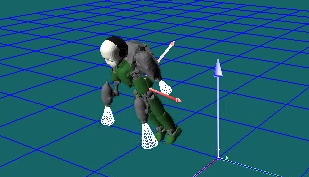
\includegraphics[width=50mm]{./imagines/pitch_down.png}}
%    \caption{a) Scenario 1; b) Scenario 2, with the aerodynamic force vector and body frame shown as arrows on the body.} 
%    \label{fig:scen}
%\end{figure}

%\begin{figure}[t]
%      \centering
%      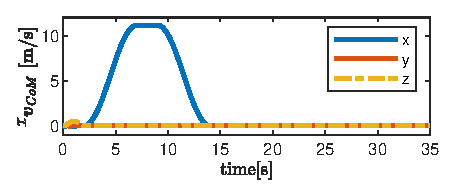
\includegraphics[width=60mm]{./imagines/vcom.eps}
%     \caption{robot's CoM velocity profile w.r.t. the inertial frame}
%     \label{fig:motion}
%\end{figure}

\subsection{Control Results for the Hovering Scenario}

\begin{figure}[t]
    \centering
        \subfigure{\label{fig:hovering_wind} 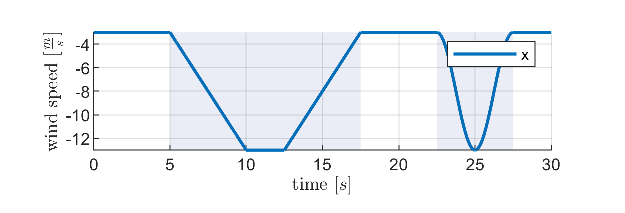
\includegraphics[width=0.97\columnwidth]{./imagines/pics_v2/wind_hov.eps}}
        \subfigure{\label{fig:hovering_angMom}
        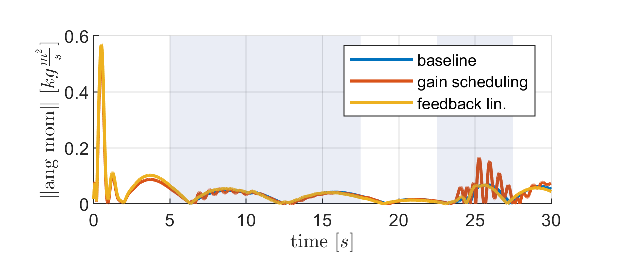
\includegraphics[width=0.97\columnwidth]{./imagines/pics_v2/angMom_hov.eps}}
        \subfigure{\label{fig:hovering_linMom}
        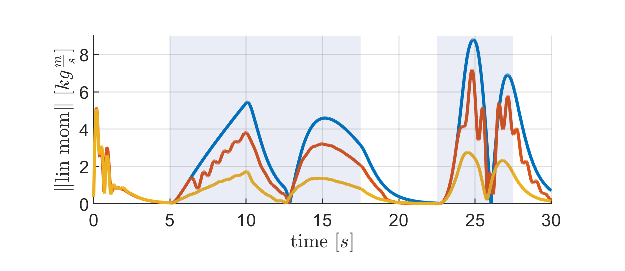
\includegraphics[width=0.97\columnwidth]{./imagines/pics_v2/linMom_hov.eps}}
        \vspace{-0.1cm}
        \subfigure{\label{fig:hovering_com}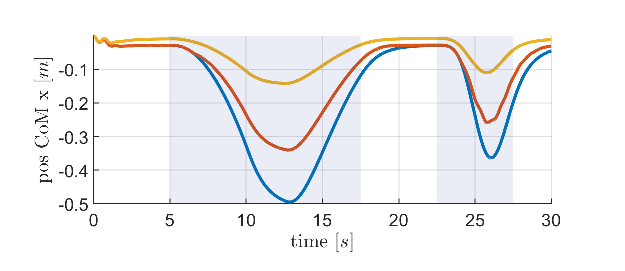
\includegraphics[width=0.97\columnwidth]{./imagines/pics_v2/posX_hov.eps}}        
        \caption[]{Hovering scenario. From top to bottom: a) wind profile; b) angular momentum error norm; c) linear momentum error norm; d) center of mass position error in the wind direction.}
        \label{fig:hovering_plots}
\end{figure}

\begin{figure}[t]
    \centering
        \subfigure{\label{fig:high_speed_wind}
        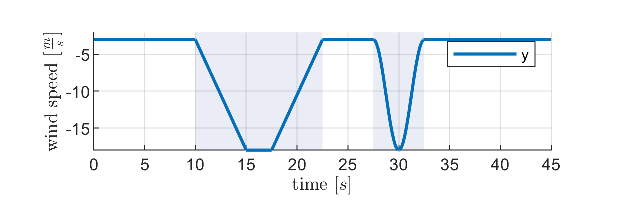
\includegraphics[width=0.97\columnwidth]{./imagines/pics_v2/wind_hspe.eps}}
        \subfigure{\label{fig:high_speed_angMom}
        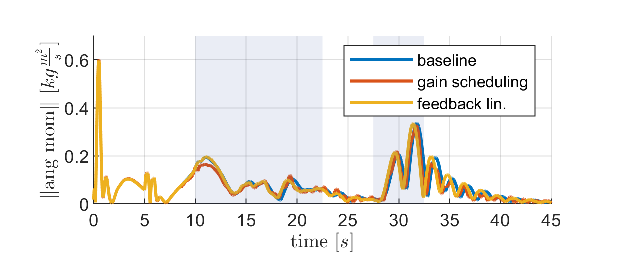
\includegraphics[width=0.97\columnwidth]{./imagines/pics_v2/angMom_hspe.eps}}
        \subfigure{\label{fig:high_speed_linMom}
        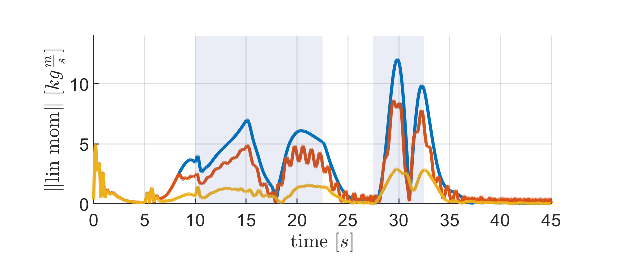
\includegraphics[width=0.97\columnwidth]{./imagines/pics_v2/linMom_hspe.eps}}
        \subfigure{\label{fig:high_speed_com}
        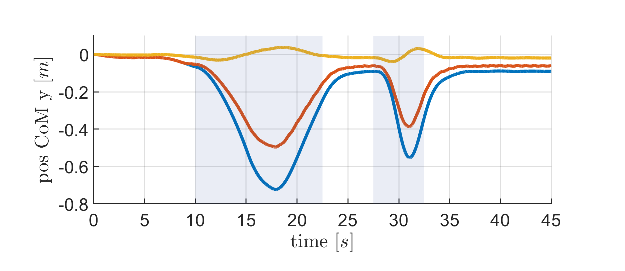
\includegraphics[width=0.97\columnwidth]{./imagines/pics_v2/posY_hspe.eps}}        
        \caption[]{High speed flight scenario. From top to bottom: a) wind profile; b) angular momentum error norm; c) linear momentum error norm; d) center of mass position error in the wind direction.}
        \label{fig:high_speed_plots}
\end{figure}

% \begin{figure}[t]
%       \centering
%       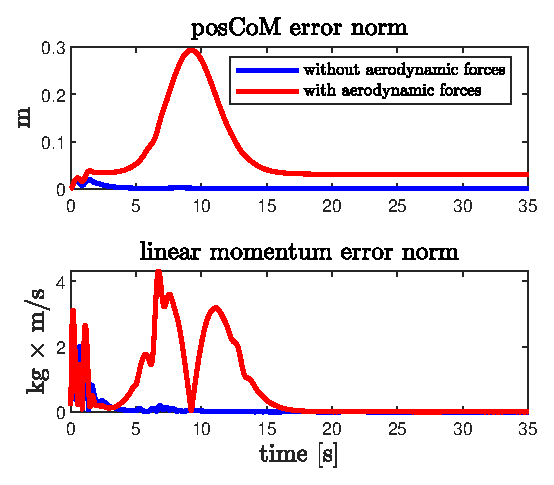
\includegraphics[width=60mm]{./imagines/pos_linMom_noaf_af.eps}
%       \caption{Hovering scenario: flight controller that does not account for aerodynamics, with (red line) and without (blue line) aerodynamic effects acting on the system.} 
%       \label{fig:h_rob} 
% \end{figure}

% \begin{figure}[t]
%       \centering
%       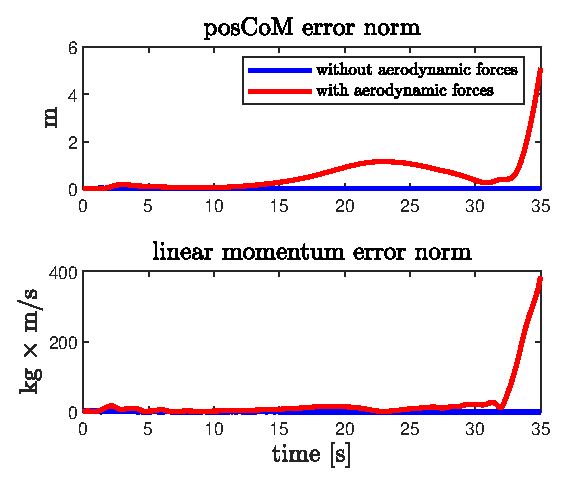
\includegraphics[width=60mm]{./imagines/pos_linMom_noaf_af_hs.eps}
%       \caption{High-speed scenario: flight controller that does not account for aerodynamics, with (red line) and without (blue line) aerodynamic effects acting on the system.} 
%       \label{fig:hf_rob} 
% \end{figure}

We evaluate the performances of three control strategies: the \emph{baseline} controller of \cite{c1}\cite{c2}, the \emph{feedback linearization} control designed in Sec. \ref{sec:control}, and a third controller that uses \emph{gain scheduling} as described in Sec. \ref{sec:control}. To test the robustness of feedback linearization controller, the aerodynamic force $F_a$ in the control model is computed assuming random noise of $\SI{5}{\%}$ and a calibration error of $\SI{10}{\%}$ on both $\alpha$ and $\beta$ angles.

Simulation results for the hovering scenario are presented in Fig.~\ref{fig:hovering_plots}, where we focused on the linear and angular momentum error norm and center of mass position error. With baseline controller, the center of mass error along the wind direction has peaks of $\SI{50}{cm}$ and $\SI{35}{cm}$ in correspondence of the wind gusts (shaded area), which are reduced by $\SI{33}{\%}$ when the gain scheduling control is used and by $\SI{71}{\%}$ for the feedback linearization control. The linear momentum error also reduces accordingly, while the angular momentum error remains comparable in all three simulations.

%At first, we performed simulations for hovering and high-speed flight conditions without considering aerodynamic forces which are the reference conditions for the analysis of aerodynamic effects on the robot, see Fig. \ref{fig:a1}, \ref{fig:c1}, \ref{fig:a2} and \ref{fig:c2}. We proceeded the robustness analysis for hovering and high-speed flight cases individually by testing the wind gust range (starting from the constant wind speed $\SI{3}{m/s}$ to the maximum wind gust value) inside which the robot can stabilize. With the wind velocity along the $-\boldsymbol{X}$ axis of the inertial frame $\mathcal{I}$, the maximum wind gust value is $\SI{53}{m/s}$ for hovering case and $\SI{9}{m/s}$ for high-speed flight. The results in Fig. \ref{fig:b1}, \ref{fig:d1}, \ref{fig:b2} and \ref{fig:d2} represent the CoM position error norm and linear momentum error norm with the air environment described in Fig. \ref{fig:wind}. The results show that with a maximum wind gust value as $\SI{10}{m/s}$, the CoM position error norm in hovering case increases evidently under the wind gust impact but it converges to equilibrium point after the wind impact; in high-speed flight case, the control outputs diverge and the robot loses stability. The limitations of current controller while handling aerodynamic effects caused by wind gust impact are pointed out.

% \begin{figure}[t]
%     \centering
%         \subfigure[]{\label{fig:a1}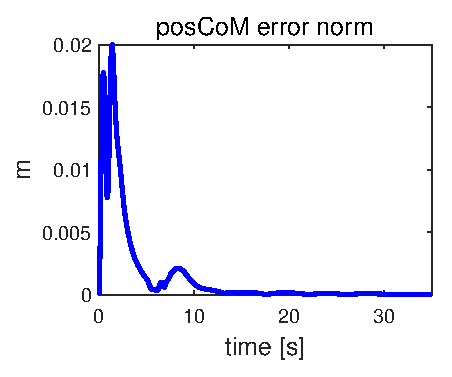
\includegraphics[width=40mm]{./imagines/pos_err_norm_h.eps}}
%         \subfigure[]{\label{fig:b1}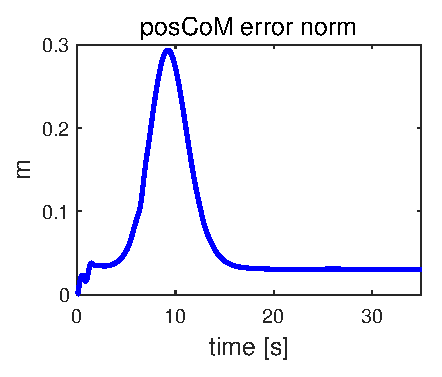
\includegraphics[width=40mm]{./imagines/pos_err_norm_0h.eps}}
%         \subfigure[]{\label{fig:c1}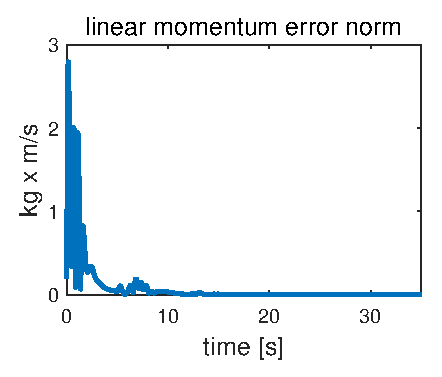
\includegraphics[width=40mm]{./imagines/linMom_err_norm_h.eps}}
%         \subfigure[]{\label{fig:d1}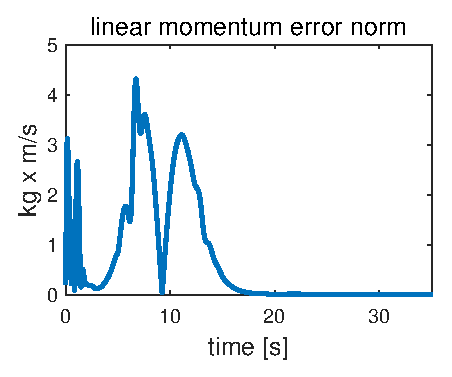
\includegraphics[width=40mm]{./imagines/linMom_err_norm_0h.eps}}
%     \caption{Hovering: a) and c) without aerodynamic effects; b) and d) with aerodynamic effects}
%     \label{fig:h_rob}
%\end{figure}
% \begin{figure}[t]
%     \centering
%         \subfigure[]{\label{fig:a2}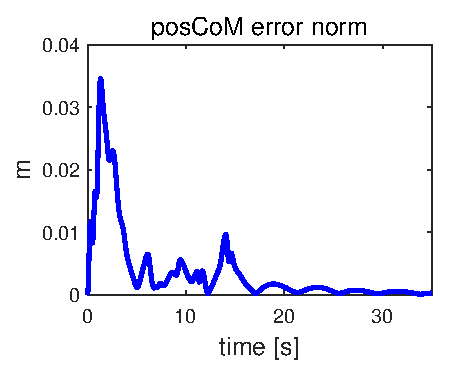
\includegraphics[width=40mm]{./imagines/pos_err_norm_f.eps}}
%         \subfigure[]{\label{fig:b2}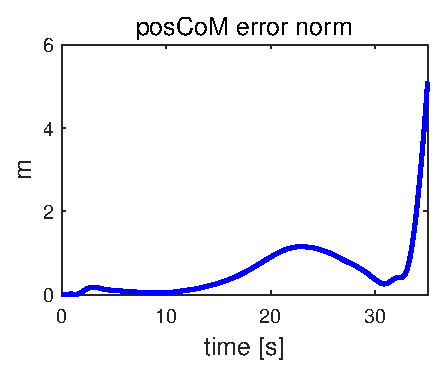
\includegraphics[width=40mm]{./imagines/pos_err_norm_0f.eps}}
%         \subfigure[]{\label{fig:c2}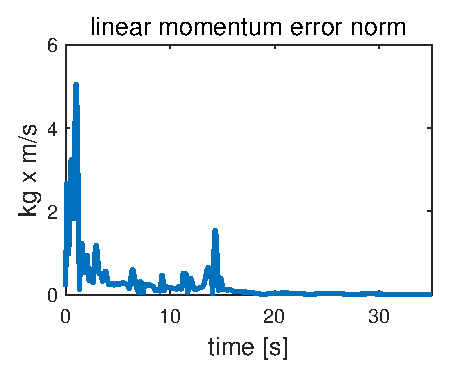
\includegraphics[width=40mm]{./imagines/linMom_err_norm_f.eps}}
%         \subfigure[]{\label{fig:d2}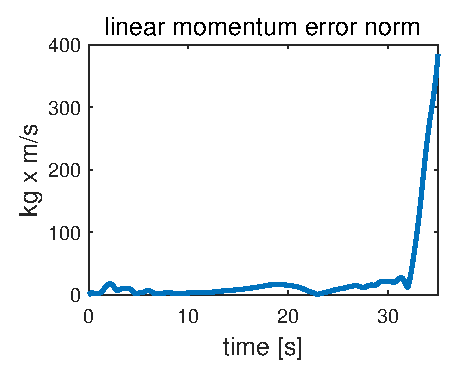
\includegraphics[width=40mm]{./imagines/linMom_err_norm_0f.eps}}
%     \caption{High-speed flight: a) and c) without aerodynamic effects; b) and d) with aerodynamic effects} 
%     \label{fig:hf_rob}
% \end{figure}

\subsection{Control Results for High Speed Flight}
\label{subsec:ctrl-results-aerodyn}

The three controllers are then tested during high speed flight. Fig.~\ref{fig:high_speed_plots} compare their performances in this second scenario: the baseline controller has the worst performances, with peaks errors on the center of mass position of $\SI{75}{cm}$ and $\SI{50}{cm}$. The gain scheduling controller is able to reduce the center of mass peaks error by $\SI{30}{\%}$, while the feedback linearization further reduces the peaks by $\SI{95}{\%}$. Linear and angular momentum errors also behave in accordance with the results already achieved for Scenario 1.

%To compare the performances of the robot with different control techniques, the air environment in the simulations is the same as in Fig. \ref{fig:wind}. The results are in Fig. \ref{fig:h_control} and \ref{fig:hf_control}, that presents the CoM position $\&$ linear momentum error norm for both hovering and high-speed flight cases implemented with gain-scheduling and feedback linearization individually. The reduction of CoM position error norm in hovering case varies quite much between the two control techniques applied; the maximum wind gust value under which the robot can stabilize during high-speed flight is increased to $\SI{10}{m/s}$ by applying gain-scheduling and to $\SI{13}{m/s}$ by applying feedback linearization. The percentage that describes the improvements of the controller is presented in Table \ref{table:comp} and the feedback control technique returns better performance in sense of overcoming the limitations of current controller considering aerodynamic effects.

%\begin{table}[t]
%\vspace*{0.3cm}
%\caption{Gain-scheduling V.S. Feedback linearization}
%\label{table:comp}
%\begin{center}
%\begin{tabular}{c|c|c}
%\toprule
%\multirow{2}{*} & Max-pos-err: & Max-wind-gust: \\ 
% & hovering & high-speed flight \\
%\midrule
%Current controller & $\SI{0.29}{m}$ & $\SI{9}{m/s}$\\
%\midrule
% Gain-scheduling  & $\SI{0.18}{m}$ ($-38\%$) & $\SI{10}{m/s}$ ($+11\%$)\\
%\midrule
%Feedback linearization & $\SI{0.035}{m}$ ($-88\%$) & $\SI{13}{m/s}$ ($+44\%$)\\
%\bottomrule
%\end{tabular}
%\end{center}
%\end{table}

%\begin{figure}[t]
%    \centering
%        \subfigure[]{\label{fig:h_control}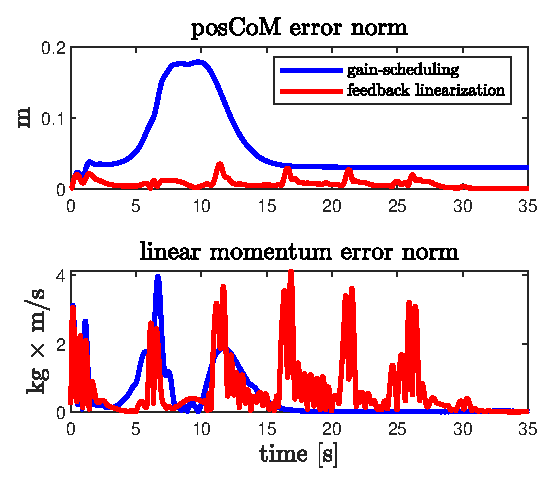
\includegraphics[width=40mm]{./imagines/pos_linMom_fl_2h.eps}}
%        \subfigure[]{\label{fig:hf_control}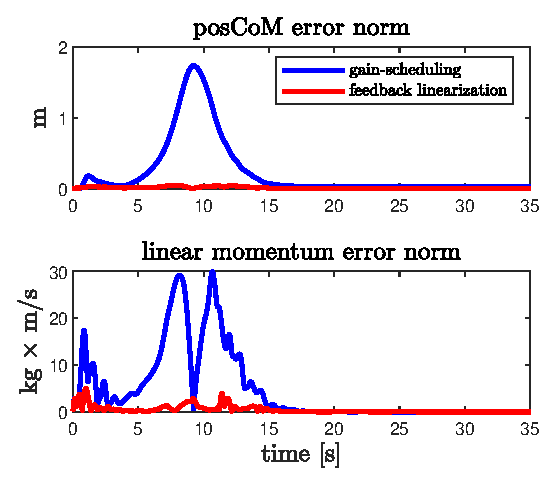
\includegraphics[width=40mm]{./imagines/pos_linMom_fl_1f.eps}}
%    \caption{a) Hovering Scenario: gain-scheduling (blue) V.S. feedback linearization (red); b) High-speed scenario: gain-scheduling (blue) V.S. feedback linearization (red).} 
%    \label{fig:fl_gs}
%\end{figure}




% \begin{figure}[t]
%       \centering
%       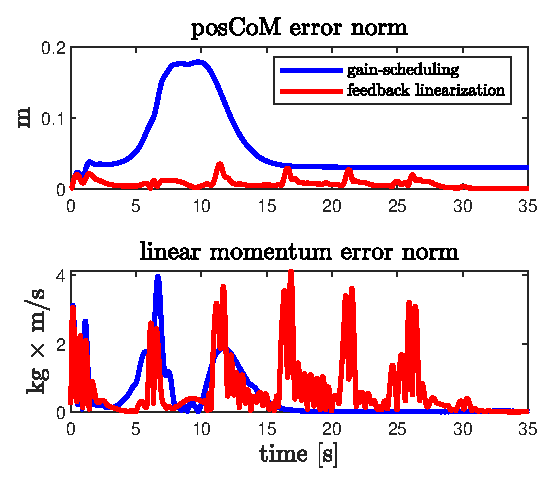
\includegraphics[width=60mm]{./imagines/pos_linMom_fl_2h.eps}
%       \caption{Hovering Scenario: gain-scheduling (blue) V.S. feedback linearization (red)} 
%       \label{fig:h_control} 
% \end{figure}

% \begin{figure}[t]
%       \centering
%       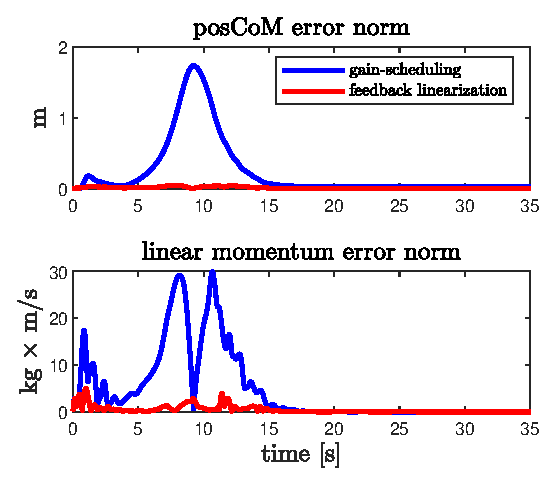
\includegraphics[width=60mm]{./imagines/pos_linMom_fl_1f.eps}
%       \caption{High-speed scenario: gain-scheduling (blue) V.S. feedback linearization (red)} 
%       \label{fig:hf_control} 
% \end{figure}

% \begin{figure}[t]
%     \centering
%         \subfigure[]{\label{fig:a3}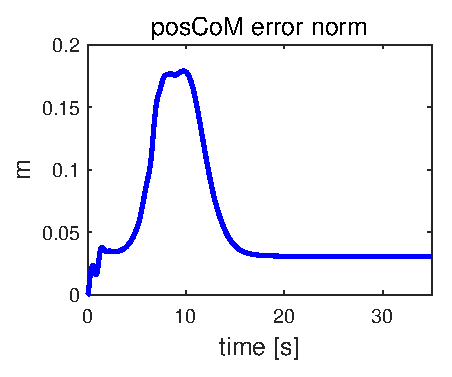
\includegraphics[width=40mm]{./imagines/pos_err_norm_2h.eps}}
%         \subfigure[]{\label{fig:b3}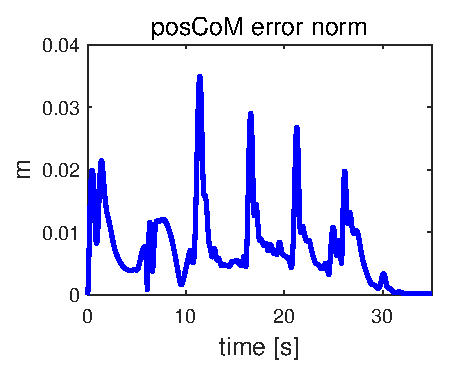
\includegraphics[width=40mm]{./imagines/pos_err_norm_fl_0h.eps}}
%         \subfigure[]{\label{fig:c3}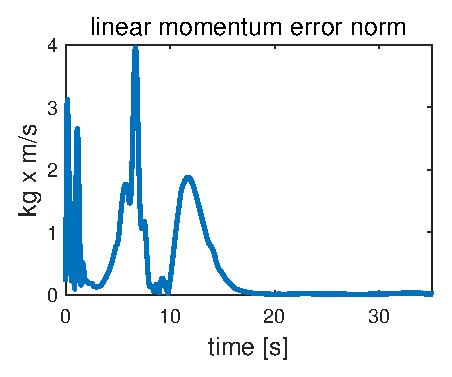
\includegraphics[width=40mm]{./imagines/linMom_err_norm_2h.eps}}
%         \subfigure[]{\label{fig:d3}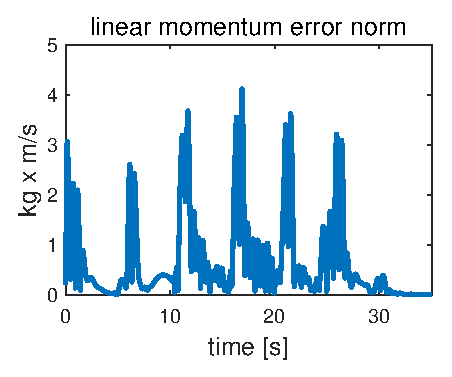
\includegraphics[width=40mm]{./imagines/linMom_err_norm_fl_0h.eps}}
%     \caption{Hovering: a) and c) gain-scheduling; b) and d) feedback linearization} 
%     \label{fig:h_control}
% \end{figure}

% \begin{figure}[t]
%     \centering
%         \subfigure[]{\label{fig:a4}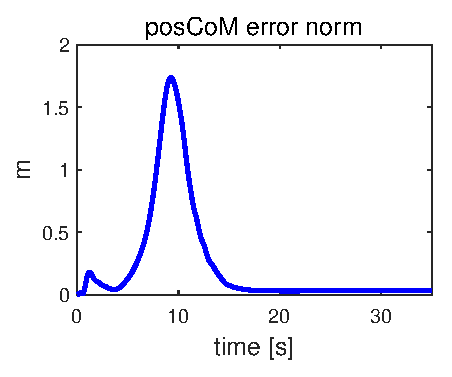
\includegraphics[width=40mm]{./imagines/pos_err_norm_1f.eps}}
%         \subfigure[]{\label{fig:b4}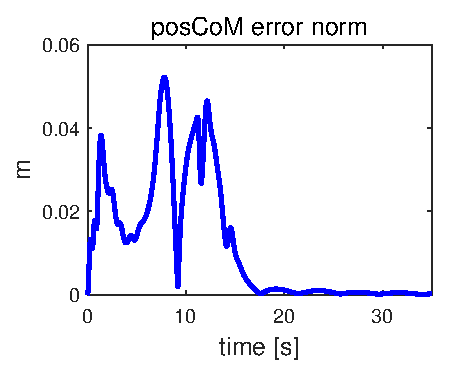
\includegraphics[width=40mm]{./imagines/pos_err_norm_fl_0f.eps}}
%         \subfigure[]{\label{fig:c4}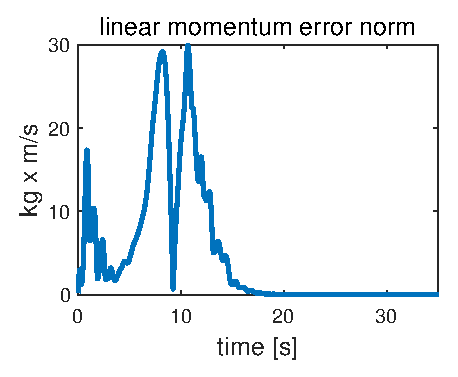
\includegraphics[width=40mm]{./imagines/linMom_err_norm_1f.eps}}
%         \subfigure[]{\label{fig:d4}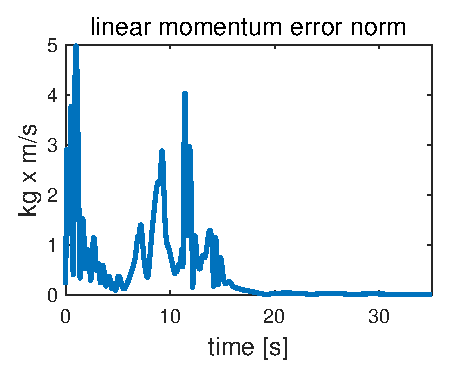
\includegraphics[width=40mm]{./imagines/linMom_err_norm_fl_0f.eps}}
%     \caption{High-speed flight: a) and c) gain-scheduling; b) and d) feedback linearization} 
%     \label{fig:hf_control}
% \end{figure}
